\documentclass{beamer}
\usetheme{Madrid}
\usecolortheme{whale}
\setbeamertemplate{navigation symbols}{}%hide navigation buttons at bottom
\usepackage[backend=biber]{biblatex}
\addbibresource{main.bib}


\title[Volatility Analysis]{What is the impact of new product announcements on the stock price volatility of major technology companies? }
\author{Dauer L. Profumo N. Tognolini B. Angevin P.}
\date{December 11, 2024}

\begin{document}

% Title Slide
\begin{frame}
  \titlepage
\end{frame}

\begin{frame}{Table of content}
\begin{enumerate}
    \item Introduction
    \item Data processing
    \item Descriptive Analysis
    \item Model
    \item Results
    \item Conclusion
    \item Bibliography
\end{enumerate}
\end{frame}

\section{Introduction}
\begin{frame}{Introduction: Theme}
  \begin{itemize}
    \item <1-> Why did we choose this topic ?
    \item <2-> We are 4 students studying finance who are interested in stock market prices. 
    \item <3-> We wanted to learn how to use IT as a tool for finance
    \item <4-> And we were wondering if there is any correlation between stock prices and product announcements in the tech industries such as Apple, Amazon, Tesla etc...
    \item <5-> Because stock volatility is a key metric for understanding market risk.
  \end{itemize}
\end{frame}
    
\end{frame}
\section{Introduction}
\begin{frame}{Introduction}
  \begin{itemize}
    \item <1-> How did we get the project done ?
    \item <2-> As everything was new for us, we first started by watching a YouTube video about what GitHub was...
    \item <3-> We successfully found out how to do our first commits and add files on GitHub (git push, git clone, etc...)
    
  \end{itemize}
\end{frame}

\begin{frame}{Introduction}
\includegraphics[width=0.9\textwidth]{}
\begin{figure}
        \centering
        \includegraphics[width=0.9\linewidth]{}
\begin{figure}
            \centering
            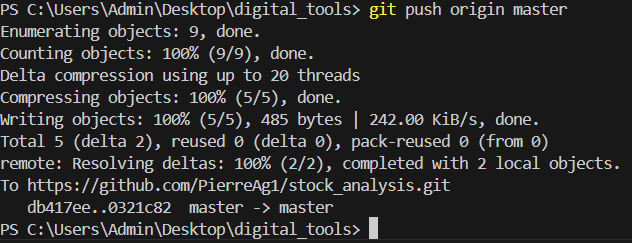
\includegraphics[width=1\linewidth]{gitpush.png}
        \end{figure}
                \caption{Successful git push command. }
        \label{fig:enter-label}
    \end{figure} 
\end{frame}


\begin{frame}{Introduction: Repository}
\begin{enumerate}
    \item <1-> README.md
    \item <2->requirements
    \item <3->.gitignore
    \item <4->Dockerfile
    \item <5->Data
    \item <6->Notebook.ipynb
    \item <7->Text
    
\end{enumerate}
\end{frame}

\begin{frame}{Introduction}
\begin{figure}
    \centering
    \includegraphics[width=1\linewidth]{Repo.png}
    \caption{Our repository on GitHub.}
    \label{fig:enter-label}
\end{figure}
    
\end{frame}


% Data Processing Slide
\section{Data}

% Example Graphic
\begin{frame}{Data importation, merging and cleaning}
  \begin{itemize}
      \item <1->After that we had to find data to work with
  \end{itemize}
    
\end{frame}

\begin{frame}{Data Processing}
  \begin{itemize}
    \item Key datasets:
      \begin{itemize}
        \item Company announcements dataset.
        \item Daily stock prices dataset.
      \end{itemize}
    \item Key pre-processing steps:
      \begin{itemize}
        \item Cleaning column names.
        \item Converting date formats.
        \item Merging stock prices with announcement data.
      \end{itemize}
  \end{itemize}
\end{frame}

\begin{frame}{Data libraries importations}
\begin{itemize}
    \item pandas for data manipulation and analysis
    \item matplotlib for creating visualisations
    \item numpy for numerical computation
    \item seaborn for enhanced statistical visualisations
    \item scikit-learn for statical modeling (linear regression) and for model validation 
\end{itemize}
    
\end{frame}

% Example Graphic
\begin{frame}{Data Cleaning Example}
  \centering
  \includegraphics[width=0.8\textwidth]{} % Placeholder for a data cleaning graph
\begin{figure}
      \centering
      \includegraphics[width=0.5\linewidth]{Capture d'écran 2024-12-01 180129.png}
      \caption{Data frame after cleaning process.}
      \label{fig:enter-label}
  \end{figure}
\end{frame}

% Example Graphic
\begin{frame}{Data Cleaning Example}
\begin{itemize}
    \item  We removed every negative values, missing values and zero values
    \item 
    \centering
  \includegraphics[width=0.8\textwidth]{} % Placeholder for a data cleaning graph
\begin{figure}
          \centering
          \includegraphics[width=0.5\linewidth]{image.png}
          \caption{Results of any missing, zero, negative values.}
          \label{fig:enter-label}
      \end{figure}
    \end{itemize}
\end{frame}

% Analysis Slide

\begin{frame}{Compute daily returs \& rolling volatility}
  \begin{itemize}
      \item <1->After the data cleaning process, we computed the daily returns and the rolling volatility for each stock 
      \item <2->\begin{figure}
              \centering
              \includegraphics[width=0.5\linewidth]{return_volatility.png}
              \caption{Results of daily return \& rolling volatility.}
              \label{fig:enter-label}
          \end{figure}
  \end{itemize}
\end{frame}

% Analysis Slide
\section{Analysis}
\begin{frame}{Compute daily returs \& rolling volatility}
  \begin{itemize}
    \item Daily returns calculated using percentage change.
    \item Rolling volatility computed using a 10-day window.
   
  \end{itemize}
\end{frame}

% Analysis Slide
\section{Analysis}
\begin{frame}{Descriptive analysis}
  \begin{itemize}
    \item <1->With this clean data frame we can now plot different graphics 
    \item <2->The announcements are represented by vertical lines on the graphic
    \item <3->The next slides shows the different graphics (with different firms and different time frames).
    
  \end{itemize}
\end{frame}

% Visualization Example
\begin{frame}{Descriptive analysis}
  
\begin{figure}
      \centering
      \includegraphics[width=1
      \linewidth]{everyfirms.png}
      \caption{All stock prices between 2014 and 2024.}
      \label{fig:enter-label}
  \end{figure}
    
\end{frame}

% Visualization Example
\begin{frame}{Rolling Volatility Visualization}
  
\begin{figure}
      
      
\begin{figure}
          \centering
          \includegraphics[width=1\linewidth]{apple2years.png}
          
          \label{fig:enter-label}
      \end{figure}
            \caption{APPL stock price between 2019 and 2020.}
      \label{fig:enter-label}
  \end{figure}
    
\end{frame}
% Results Slide
\section{Results}
\begin{frame}{Results}
  \begin{itemize}
    \item Pre- and post-announcement volatility changes were computed.
    \item Average changes in 10-day rolling volatility due to announcements:
      \begin{itemize}
        \item Significant increases observed for Company A.
        \item No significant change for Company B.
      \end{itemize}
  \end{itemize}
\end{frame}

% Regression Results Slide
\begin{frame}{Linear Regression Results}
  \begin{itemize}
    \item A binary variable for announcements was introduced.
    \item Regression results:
      \begin{itemize}
        \item Intercept: \texttt{value from your notebook}.
        \item Coefficient: \texttt{value from your notebook}.
      \end{itemize}
    \item R-squared: \texttt{value from your notebook}.
  \end{itemize}
\end{frame}

% Conclusion Slide
\section{Conclusion}
\begin{frame}{Conclusion}
  \begin{itemize}
    \item Volatility analysis provides insights into market reactions to company announcements.
    \item This project combines data processing, statistical analysis, and visualization.
    \item Future work:
      \begin{itemize}
        \item Expand analysis to include more companies.
        \item Improve modeling techniques to predict volatility more precisely.
      \end{itemize}
  \end{itemize}
\end{frame}

\begin{frame}{Bibliography}
    
\end{frame}
\end{document}
